\chapter{Graph Neural Networks (GNNs)} \label{GNN}

\section{Introduction}

Real world entities are often defined by their connections to other
objects. These objects together with their connections define
\textit{graphs} as described in \sref{sec:graphs}. In the past decade,
research has been conducted in neural networks \cite{article:TGNNM}
which can operate in graph data; vertices, edges and global attributes
of graphs. Graphs can express systems organized in a large number and
interacting, and complex systems, which can be found in various areas
of scientific study. As a defining characteristic, GNNs are deep
learning methods operating on the graph domain \cite{article:zhou}.

Historically, interest in neural networks for graph structured data
appeared with applications of RNNs at the end of the 20th century
\cite{article:sperduti}. The revolution that CNNs brought to the
scene of deep neural networks resulted in a rekindled interest for
GNNs at the start of the last decade, as they have the ability to
extract localized spatial features and construct expressive representations.

While the architecture of CNNs allowed for breakthroughs on data which
is organized in euclidean space, such as images (2D grid) or
one dimensional sequences (text or speech), it is hard to express
graphs on an euclidean domain, as generally, graphs are non-Euclidean.
An effort to extend structured deep learning models to non-Euclidean
domains, such as in graphs or manifolds, is underway and it is called
\textit{geometric deep learning}\cite{article:geomDeep}. 

Another research approach is focused on \textit{graph representation
  learning} \cite{hamilton2017representation, article:zhang} which aims
to translate and represent graphs, nodes and edges as low-dimensional
vectors thereby preserving network topology structure, vertex content
and other graph level information. This approach is based on the idea
of \textit{representation learning} which was sparked by the work done
by \textit{Mikolov et al.} in 2013 in word embedding
\cite{mikolov2013efficient,mikolov2013distributed}, widely regarded
as the first graph embedding method based on representation learning.
In this thesis, graph representation learning techniques
were used.

Recently, the expressive power of GNNs has found practical use in
several scientific application such as drug discovery
\cite{article:xiong,article:bognini}, molecular properties prediction
\cite{article:wieder}, physics aware simulations \cite{article:sanchez},
applications in (internet) network intrusion detection \cite{article:weng},
spammer detection in cyberspace \cite{article:zhiwei}, anomaly
detection in social networks and email networks \cite{article:chaudhary},
fake news detection \cite{article:monti}, traffic forecasting \cite{article:jiang}
and many more. 

GNNs take into account the features of the underlying graphs
and can make informed decisions about them, either in classification
or prediction tasks, matching or surpassing the capabilities of older methods
such as graph kernels and random walk methods \cite{xu2018powerful}.

Some examples of data that is suitable for representation in
a graph structure and commonly studied in literature are presented
below:

\begin{itemize}
\item
  \textbf{Molecules}. Molecules constitue an excellent example
  of an entity that can be represented with a graph, as they consist of
  atoms (nodes) that are connected with bonds (edges) and they can
  have several molecular properties (global properties). It is a
  very common abstraction in literature, even before the advent of
  GNNs, to represent them in this structure\cite{article:duvenaud}.
  \begin{figure}
    \centering
    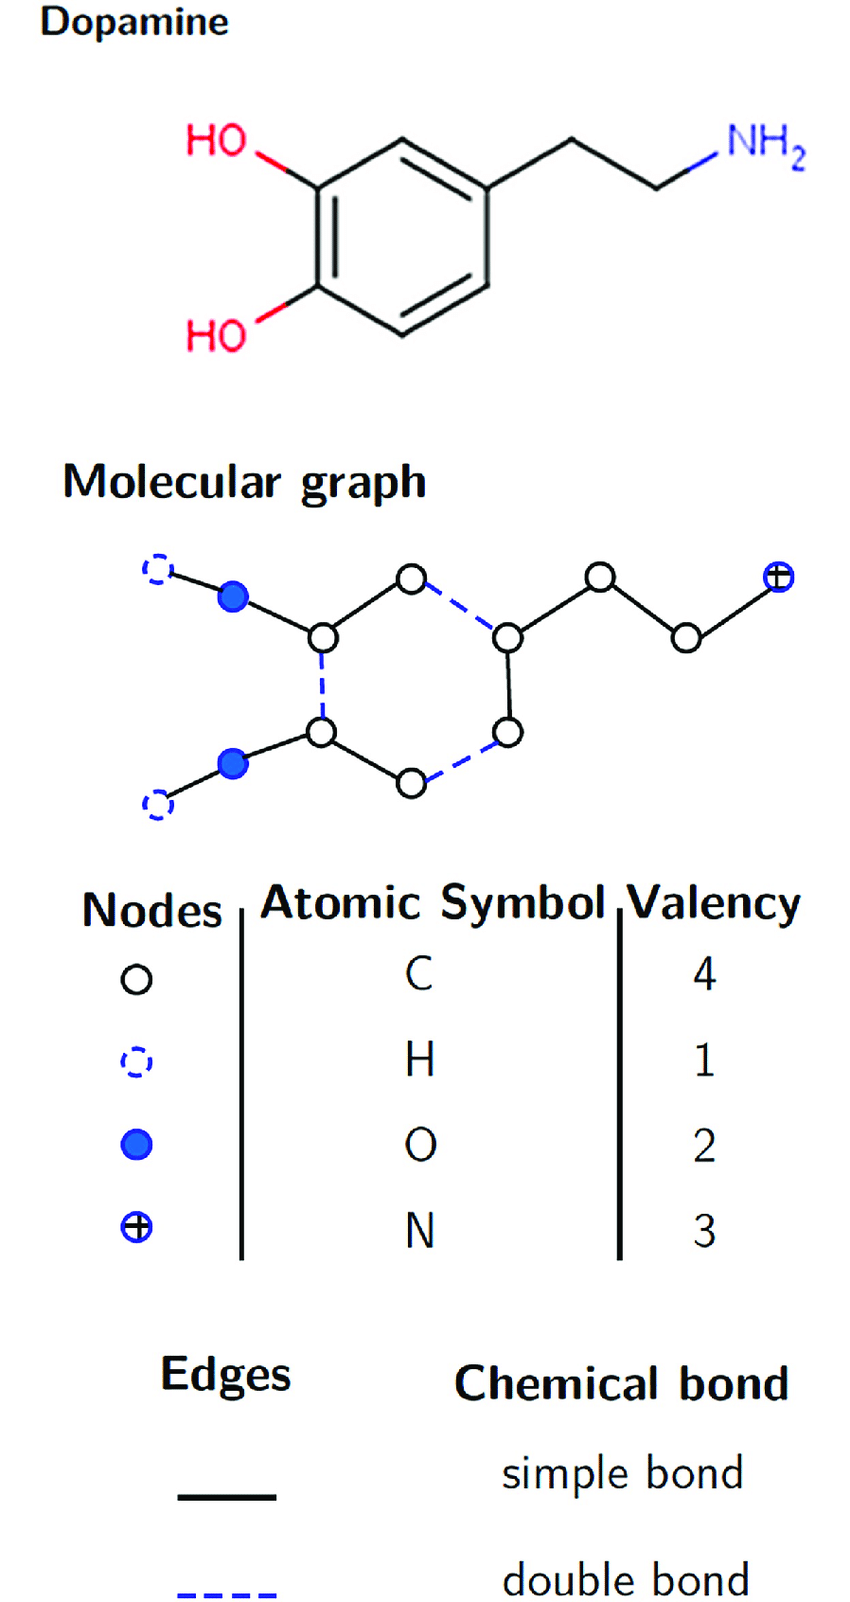
\includegraphics[width=0.4\textwidth]{Figures/chap_gnn/dopamine.png}
    \caption{Dopamine molecule represented as a graph. Different types of nodes represent different atoms and different edges represent the chemical bonds present in the molecule. Image source \citet{article:stefi}.}
    \label{fig:dopamine}
  \end{figure}
\item
  \textbf{Social Networks}. Social networks are networks between
    social actors who interact with each other. These types of networks
    are important when studying patterns of collective behaviour or even
    epidemics and other social phenomena.. In this
    representation, it is common to represent actors as nodes and their
    relationship as edges.
  
\end{itemize}


\subsubsection*{Tasks}
The tasks that a GNN can be used to accomplish can be
divided in three main categories, graph (or master) level, node level and edge level.
\begin{itemize}
\item
  \textbf{Graph-level task}. These types of tasks operate
  on the global (or master) node, and can be used to classify
  or predict some of their properties. For example, when representing
  a molecule as a graph, they can be used to indicate whether it is toxic,
  or in social networks when applying some opinion dynamics models it can
  indicate if a network has reached concesus.

\item
  \textbf{Node-level task}. Node level tasks predict or classify some
  properties or the role of nodes in a graph. As an example, in a model
  used in studying a simple SIS dynamics, node level tasks would predict
  the state of the node.
\item
  \textbf{Edge-level task}. Edge level tasks predict or classify edge
    properties or even predict the existence of an edge between two nodes
    (\textit{link prediction}). In the latter case, it is common to consider
    a graph fully connected and then prune edges to arrive to a sparse graph.
\end{itemize}

\section{From CNNs to Graph Neural Networks}

\subsection{Challenges}

\textbf{Structure} As discussed previously, CNNs are extremely efficient at extracting
spatial features and creating effective representations from the input data.
This is useful when input data is topologically static, as in the
case of images, but graphs are flexible mathematical models, where
the input data \textbf{lacks consistent strucure} makes creating useful
representations difficult. For instance, consider the task of predicting 
whether a molecule is toxic; molecules may have different numbere of atoms,
which may be of different types, each connected with a different number of
nodes of different types (ionic, covalent and of different strength).


\textbf{Node-order equivariance} Images have a two-dimensional structure
where each pixel is defined by its absolute position within the image, possibly
even defining features based on itself and its neighborhood. In graphs, nodes
have no inherent ordering and thus any possible representation should not
depend on the order of the nodes --- permutations on node ordering
should result in representation that reflect the same outputs.

\textbf{Scalability} Networks can be huge, i.e. a graph of the users
of social networks could number billions of nodes and connections.

\subsection{Creating embeddings}

Before moving to convolutions on graphs and other forms of
neural networks, a representation of the graph in embedding space
must be created, which maps individual nodes to fixed-sized
real value vectors. This allows the application of modern  machine
learning algorithms, designed for sequences of data or grid-topology
to be applied on graphs. The goal of this procedure is to encode nodes
so the similarity in the embedding space approximates the similarity in
original network. Typically, node embedding consists of three basic
stages:
\begin{enumerate}
\item
  An encoder $ENC$ is defined which maps nodes i.e. $u$ and $v$ to
  low-dimensional vectors $z_u$ and $z_v$.
  \begin{figure}[H]
    \centering
    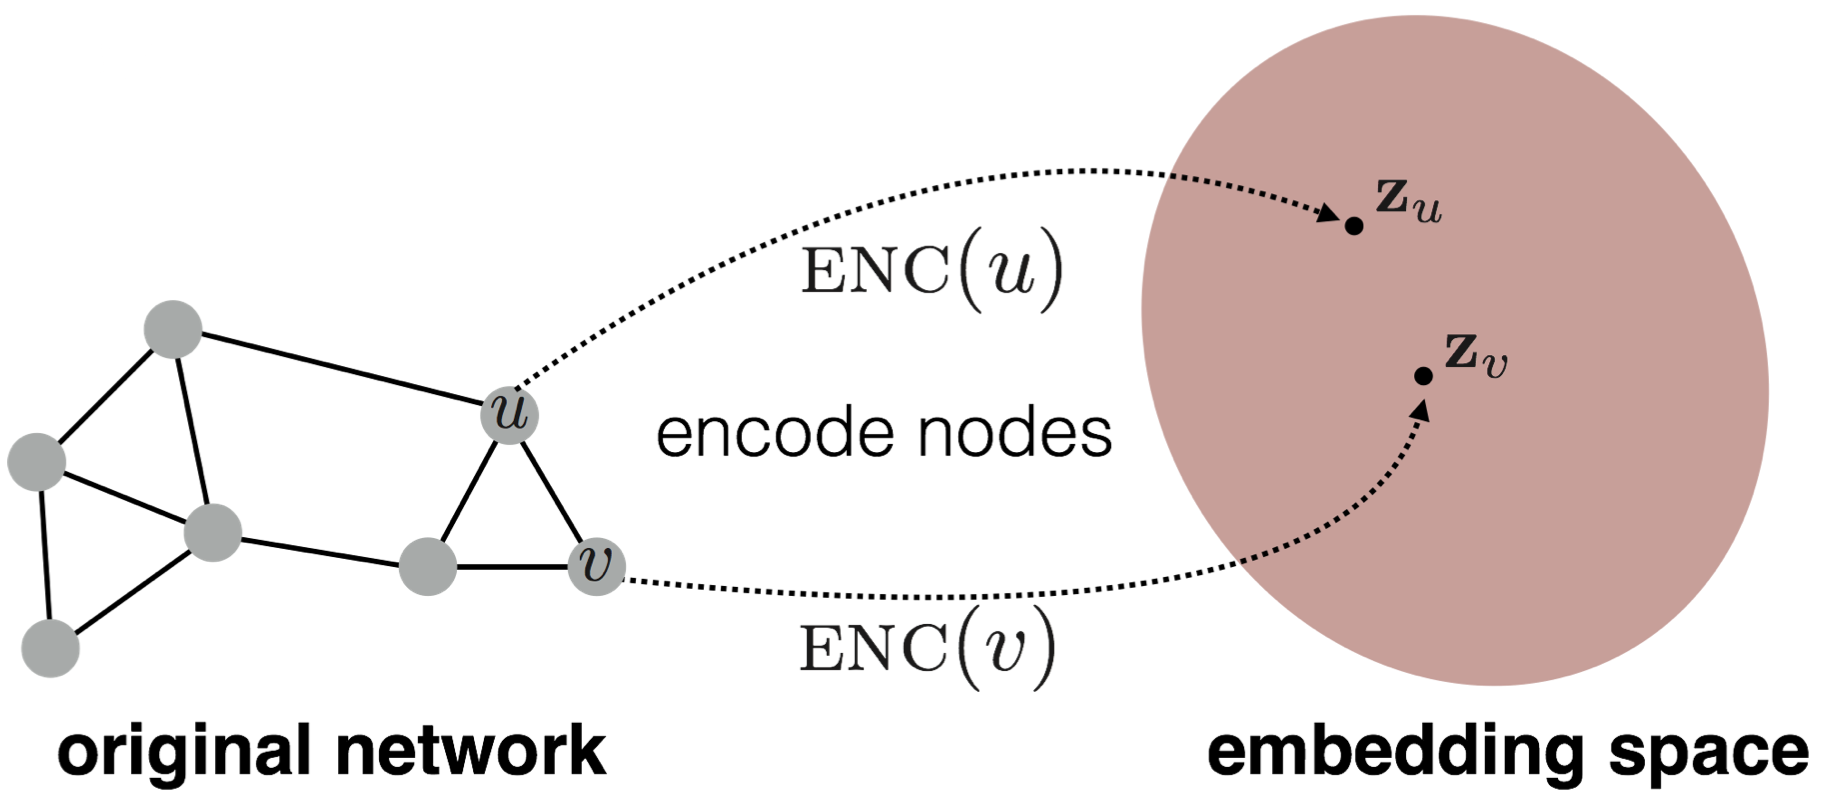
\includegraphics[width=0.6\textwidth]{Figures/chap_gnn/nodeEmbeddings.png}
    \caption{Embedding of nodes $u$ and $v$ to low dimensional vector space. Image source \cite{site:embeddings}}
    \label{fig:node_embedding}
  \end{figure}
\item
  A node similarity function $F_{sim}$ is defined which specifies how the relationships
  in the original network map to these in the vector space.
\item
  The parameters of the encoder are optimized so that the
  similarities in the original network are approximately the same
  as the dot product of the node embeddings: $F_{sim}(u,v) \approx \bm{z_u}^\intercal \bm{z_v}$
\end{enumerate}

In the following section several types of embedding methods will be
showcased. The notation $h_v^{(k)}$ denotes the representation of node
$v$ after $k$ iterations\footnote{Iterations in this case can be
thought as layers, which were discussed in previous sections.} of the
algorithms. Nodes have individual features as part of their input,
where $x_v$ denotes the $x$ feature of the $v^{th}$ node.
\begin{figure}[H]
   % \centering
     \begin{subfigure}[c]{0.4\textwidth}
         \centering
         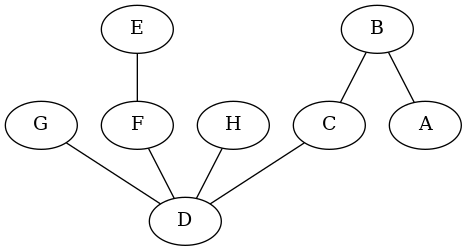
\includegraphics[scale=0.5]{Figures/chap_gnn/edge_features.png}
  \label{fig:feature_map}
     \end{subfigure}
     \hfill
     \begin{subfigure}[c]{0.4\textwidth}
       \centering
$ \begin{matrix}
A & 1 \\
B & 4 \\
C & 3 \\
D & 7 \\
E & 3 \\
F & 2 \\
G & 1 \\
H & 9 
  \end{matrix}  $
\end{subfigure}
\caption{A graph and its corresponding feature vector. The feature
  vector contains the features from all the nodes, in this case simply
a real number.}
\label{fig:combo_feature}
\end{figure}

\subsection{Initial Implementations}

In this section an introduction to the methods used for embedding
will be made, at first mentioning the polynomial methods used
historically before moving to modern graph neural network techniques.

\textbf{Polynomials of the graph Laplacian}


The graph Laplacian was discussed in \sref{sec:laplacian} while the use of its
polynomials as a means of creating embeddings was first suggested
by \citet{defferrard2016convolutional} in 2016. According to this
publication, it is possible to define polynomials of the form:
\begin{equation}
  \label{eq:polynomial_basic}
  p_w(L) = w_0 I_n + w_1L + w_2L^2 + \cdot + w_dL^d = \sum_{i=0}^dw_iL^i
\end{equation}

where $w = [w_0, \cdot w_d]$ is a vector of coefficients. Each $w$,
$p_w(L)$ and $L$ are $n\times n $ matrices.

A feature vector's $x_v$  convolution can then be written as:
\begin{equation}
  \label{eq:convo_pol}
  x' = p_w(L) x 
\end{equation}

For instance, considering the convolution of a node $v$
with $w_1 = 0$ and all other coefficients equal to 0:
\begin{equation}
  \begin{split}
  x'_v &= (Lx)_v = L_v x \\
 &= \sum_{u \in G}L_{vu}x_u \\
 &= \sum_{u \in G}(D_{vu} - A_{vu})x_u \\
 &= D_vx_v - \sum_{u\in N(v)} x_u
  \end{split}
  \label{eq:conv_ex}
\end{equation}

It possible to show \cite[Lemma ~5.2]{article:hammond} that the
degree $d$ of the polynomial directly influences the behaviour of the
convolution as:
\begin{equation}
  \label{eq:poly_deg}
  \text{dist}_G(v,u)>i \rightarrow L^i_{vu} = 0
\end{equation}

which implies that the convolution of $x$ with a
polynomial of degree $d$ is:
\begin{equation}
  \label{eq:poly_fin}
  x'_v = \sum_{i=0}^dw_i \sum_{\substack{u \in G \\ \text{dist}G(v,u) \leq i}} L^i_{vu}x_u
\end{equation}

This means that the node $v$ convolves with nodes $u$ which are up to distance $d$; thus
this creates localized filters with a degree governed completely by $d$. Note that a
direct comparison with CNNs leads to the conclusion that the polynomials are in a sense
equivalent to filters, and the weights used in previous equations are the (shared) weights
of these filters.

Another variant of this polynomial method is called ChebNet
\cite{defferrard2016convolutional} and replaces the filters with the
Chebyshev polynomials of the first kind.
% \textbf{ChebNet}
\begin{remark}
  \textbf{Order equivariance of polynomial filters}

  The polynomial filters of the previous section are order equivariant, a fact
  which is easy to prove. Considering the permutation matrix \footnote{
    A permutation matrix is a square binary matrix which has exactly one
    entry of 1 in each row and column and 0 elsewhere. 
  } $P$, an algorithm $f$ is node-order equivariant if and only if for all
  permutations of $P$:
  \begin{equation*}
    f(Px) = Pf(x)
  \end{equation*}
  Following the transformations:
  \begin{equation*}
    \begin{split}
      x & \rightarrow Px\\
      L & \rightarrow PLP^\intercal\\
      L^i & \rightarrow PL^iP^\intercal
    \end{split}
  \end{equation*}
  the polynomial filter equation changes as:
  \begin{equation*}
    \begin{split}
      f(Px) & = \sum_{i=0}^dw_i (PL^iP^\intercal)(Px) \\
            & = P \sum_{i=0}^d w_iL^ix' \\
            & = Pf(x)
    \end{split}
  \end{equation*}
  thus it is node-order equivariant.
  \end{remark}


\subsubsection{Algorithmic Computation using polynomials}

A neural network using stacked layers of any kind of polynomial filter
can be created, much like a CNN. For $K$ different polynomial filter layers,
each gets a vector $\bm{w^{(k)}}$ of learnable weights. The operation starts
  from an initial vector of features $x$.
\begin{algorithm}
\caption{Embedding Computation for a GNN using $K$ polynomial filter layers.}
\label{alg:embedding_comp}
\DontPrintSemicolon
\KwData{A feature vector $x$}
\KwResult{An embedding for $K^{th}$ }
\Begin{
  % layers = $1, 2, 3, ... L$\;
  \tcp{Vector of initial features.}
  $h^{(0)} \gets x$\;
  $layers \gets [1, 2, \dots K]$\;
  \For {k in layers}{
    \tcp{The polynomial matrix $p^{(k)}$ is computed and multiplied with last embedding}
    $p^{(k)} \gets p_{w^{(k)}}(L)$\;
    $g^{(k)} = p^{(k)} \times h^{(k-1)}$\;
    \tcp{$g$ goes through a non-linear activation $\sigma$}
    $h^{(k)} \gets \sigma (g^{(k)})$\;
    
    
  }
}
\end{algorithm}

Note that this computation can be thought as ``message passing'' between
connected nodes \cite{article:messageP}, in effect each node receiving some
information from its neighbors. Some analogies to the CNNs should better explain
the concept of message passing; the iterative nature of this method, i.e. repeating
1-hop localized convolutions K-times, is in effect the receptive field of the convolution
with each hop adding the information from another hop up to K hops away. Additionaly,
the filter weights are shared accros all the convolutions in the same manner as in
CNNs.


\section{Modern Graph Neural Networks}

\subsection{Embeddings}

Message passing forms the basis of all modern GNNs, while in this
thesis a model employing an attention layer was used, called Graph
Attention Networks first proposed by \citet{velickovic2017graph}.  The
attention \cite{article:attention} mechanism used in this paper is
briefly discussed in \aref{sec:transformers} and in the case of
graphs, it operates by computing the hidden representations of each
node by attending over its neighbors, using self-attention.

As mentioned in the previous section, a function which creates
the representations of nodes must be permutation invariant. As an
example, it is possible to consider a weighted sum as an aggregation
of a node with its first degree neighbors. A choice for a permutation
invariant function is a scalar scoring function $f(n_i, n_j)$ that
assigns weights based on pairs of nodes, scoring their relevance.
A softmax function \footnote{ A softmax (also known as softargmax or
  multi-class logistic ) function takes a vector $\bm{z}$ of real values
  as input and returns a a vector $K$ of real values that sum to 1. It
  is a generalization of the logistic function to multiple dimensions and
  its formula is $\sigma(\bm{z})_i = \frac{e^{z_i}}{\sum_{j=1}^K e^{z_j}}$
  where $K>1$.
} can be applied to focus on the neighbor with the highest relevance to the
node. A common scoring function is the inner product and it is also usual
to transform the nodes before scoring into key and query vectors to increase
the expressivity of the mechanism. 

\begin{figure}[H]
  \centering
  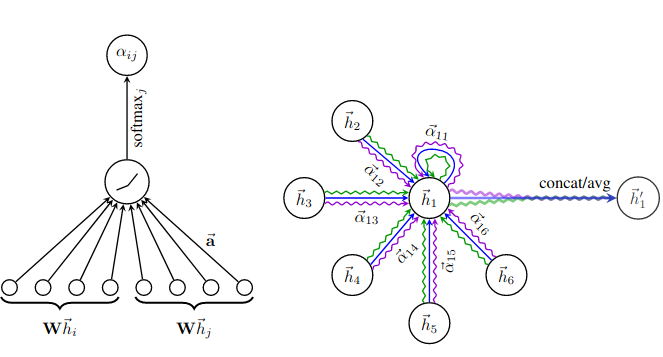
\includegraphics[width=0.75\textwidth]{Figures/chap_gnn/multiheadgat.png}
  \label{fig:multiheadGAN}
  \caption[Multi-head attention mechanism for representation
extraction]{The attention mechanism used by
\citet{velickovic2017graph}. On the \textbf{left} is a demonstration
of the attention mechanism $f(\bm{W}\vec{h}_i, \bm{W}\vec{h}_j) $ used
by the model, with a parametrization of $\bm{\vec{a}}$ of the weight
vector. On the \textbf{right} a demonstration of the multi-head module
in action, acting on node $\vec{h}_1$ with $K=3$ with independent
attention computations visible. The representation $\vec{h}'_1$ is
obtained through the aggregation of features after proper
concatenation of the heads. }
\end{figure}

The attention mechanism used in graph attention networks is extensively
discussed in \aref{sec:attentionGAT}. In a more compact form, it is possible
to express the embedding produced by a GAT in a compact form as:

Starting from $h_v^{(0)} = x_v$ for the initial embedding for node $v$:
\begin{equation}
h_v^{(k)} = f^{(k)} \Big( \bm{W}^{(k)}\Big[ \sum_{u\in
N_u}\alpha^{(k-1)}_{vu}h^{(k-1)}_u +
\alpha_{vv}^{(k-1)}h_v^{(k-1)}\Big] \Big), v \in V.
\label{eq:gat_compact}
\end{equation}

The attention weights $\alpha^{(k)}$ derivation can be found in the
appendix. Obviously, predictions can be made using the final embedding
$\hat{y}_v = g(h_v^{(K)})$ where $g$ is generally another neural network
learned together with the GAT model. The parameters $f^{(k)}, \bm{W^{(k)}} \text{and}
\bm{A^{(k)}}$ are shared across all nodes and are potentially learnable \cite{daigavane2021understanding}.

\subsection{Learning}

In the previous section, embeddings were created for nodes, using the
GAT spatial computation described. These embedding layer can be attached
in an end-to-end fashion in the same manner as a typical NN, to train the
network and produce usable outputs. This can be achieved by defining a suitable
loss function for each learning task:

\textbf{Node classification}: In a similar manner as in other classification
tasks, node classification can take advantage of the categorical cross-entropy loss
function:
\begin{equation}
  \label{eq:categoricalCE}
  L(y_v,\hat{y_v}) = - \sum_c y_{vc} log\hat{y}_{vc}
\end{equation}
where $\hat{y}_{vc}$ is the predicted probability of node $v$ belogning to class $c$.

\textbf{Graph Classification}: The aggregate of the node embeddings can be
used to create a vector representation of the entire graph which can be used
for tasks even beyond classification. It can be passed to another neural
network $NN_G$ as:
\begin{equation*}
  h_G = NN_G(AGG_{v\in G}({h_v}))
\end{equation*}

\textbf{Edge Prediction}: GNNs can be used to predict the presence or absence of
edges between nodes, by sampling pairs of adjacent and non-adjacent nodes. A loss
function closely resembling the logistic regression can be used in this case:
% \begin{equation*}
%   L(y_v, y_u, e_{vu}) = -e_{vu} log(p_{vu})
% \end{equation*}

while there are many publications on powerful pooling techniques \cite{zhang2018end,ying2018hierarchical,lee2019self}.